%%
%% CS 550 — Massive Data Mining and Learning
%% Project report (Option 1: Recommender System)
%%
%% Template class: ACM acmart (same family as the course-linked Overleaf template:
%% https://www.overleaf.com/latex/templates/acm-conference-proceedings-primary-article-template/wbvnghjbzwpc)
%%
%% Compile: pdflatex CS550_project_report.tex  (run twice if references shift)
%% Requires: acmart (TeX Live / MiKTeX). On Overleaf, start from the ACM template project
%% and replace the main .tex body with this file, or upload this file as main.tex.
%%
\documentclass[sigconf,nonacm]{acmart}

\usepackage{booktabs}
\usepackage{graphicx}
\usepackage{placeins}
\usepackage{pgfplots}
\usepackage{xspace}
\usepackage{url}
\pgfplotsset{compat=1.18}

\newcommand{\Course}{CS 550: Massive Data Mining and Learning\xspace}

\title{Recommender System for Sparse E-Commerce Ratings:\\
Amazon Arts, Crafts \& Sewing (5-core)}

\author{Nithik Pandya}
\email{nithik.pandya@rutgers.edu}
\affiliation{%
  \institution{Rutgers University--New Brunswick}
  \city{New Brunswick}
  \state{New Jersey}
  \country{USA}
}

\author{Ayush Dodia}
\email{ayush.dodia@rutgers.edu}
\affiliation{%
  \institution{Rutgers University--New Brunswick}
  \city{New Brunswick}
  \state{New Jersey}
  \country{USA}
}

\author{Vraj Shah}
\email{vraj.shah@rutgers.edu}
\affiliation{%
  \institution{Rutgers University--New Brunswick}
  \city{New Brunswick}
  \state{New Jersey}
  \country{USA}
}

\renewcommand{\shortauthors}{Pandya, Dodia, and Shah}

\begin{document}

\begin{abstract}
We build a recommender system project on the \emph{Amazon Arts, Crafts \& Sewing} 5-core dataset ($\sim$56{,}210 users, $\sim$22{,}917 items, $\sim$494{,}485 ratings, $\sim$99.96\% sparsity) by refactoring a course baseline into explicit \emph{rating prediction}, \emph{ranking}, \emph{recommendation}, and \emph{post-hoc analysis} stages. The rating branch preserves popularity and matrix factorization for MAE/RMSE evaluation, while the Top-$N$ branch preserves popularity, custom PyTorch BPR/WARP, and \texttt{implicit} BPR/ALS for Precision@10, Recall@10, F1, and NDCG@10. On top of these baselines, we add a practical counterfactual explanation layer that surfaces supporting history items, similar support items, confidence scores, and approximate weakening conditions for each recommendation. We further add an optional score adjustment layer, beyond-accuracy evaluation (coverage, diversity, novelty, and popularity concentration), a fairness audit over activity buckets, an explicit cold-start benchmark, and an optional content-aware hybrid reranker based on TF--IDF review profiles. The resulting system preserves baseline behavior while making the pipeline more modular, more explainable, and easier to report and demonstrate.
\end{abstract}

\keywords{recommender systems, collaborative filtering, matrix factorization, BPR, WARP, implicit feedback, explainability, counterfactual recommendation, fairness audit, cold-start recommendation}

\maketitle

\section{Introduction}
Online marketplaces expose users to enormous catalogs while each user interacts with only a tiny fraction of items, producing extremely sparse user--item matrices. In that setting, \emph{rating prediction}, \emph{ranking}, \emph{Top-$N$ recommendation}, and \emph{explanation} are related but distinct tasks. A model that minimizes squared error on ratings can still rank poorly at small $K$, and a ranker that produces useful Top-$N$ lists may still be opaque to end users.

Our goal in this project is therefore twofold. First, we preserve the working collaborative-filtering baseline required for \Course project \emph{Option~1}. Second, we upgrade it into a cleaner project pipeline with explicit stage boundaries, post-hoc explainability, and richer evaluation beyond average ranking accuracy. Concretely, we keep matrix factorization for rating prediction, keep popularity/BPR/WARP/implicit ALS for ranking, and add modular layers for counterfactual explanation, score adjustment, fairness auditing, beyond-accuracy diagnostics, hybrid reranking, and cold-start analysis.

\noindent\textbf{Main contributions.}
\begin{itemize}
  \item We refactor the baseline into explicit preprocessing, rating, ranking, recommendation, and analysis stages.
  \item We add a post-hoc counterfactual explanation layer with support evidence, confidence scores, and weakening conditions.
  \item We extend evaluation with beyond-accuracy, fairness, and cold-start benchmarks instead of reporting only average ranking accuracy.
  \item We add an optional content-aware hybrid reranker that can be compared directly against the same collaborative candidate pool.
  \item We expose the full pipeline in a Streamlit demo so users can inspect candidates, recommendations, explanations, and reranking behavior interactively.
\end{itemize}

\section{Related Work}
\textbf{Collaborative filtering and latent factors.} Matrix factorization and bias terms are standard for rating prediction on sparse user--item matrices~\cite{koren2009matrix,herlocker2004evaluating}. \textbf{Implicit feedback and pairwise ranking.} Consuming or ``liking'' an item is often modeled as implicit positives; Hu et al.\ propose ALS-style factorization for implicit datasets~\cite{hu2008collaborative}, while Rendle et al.\ introduce BPR for personalized ranking from implicit pairwise preferences~\cite{rendle2009bpr}. Weston et al.'s WSABIE family motivates sampled hinge/ranking losses that emphasize the top of the list~\cite{weston2011wsabie}. \textbf{Neural recommenders.} Neural collaborative filtering~\cite{he2017neural} remains a common deep-learning baseline we do not train here but cite as contrast. \textbf{Reviews and explainability.} Joint modeling of ratings and review text on Amazon-style data dates to hidden-factor topic models~\cite{mcauley2013hidden}. Our demo uses lightweight \emph{post-hoc} text overlap (TF--IDF and sentence embeddings~\cite{reimers2019sentence}) over concatenated review metadata and language for transparency rather than intrinsic model explanations; see surveys on explainable recommendation~\cite{zhang2020explainable}. \textbf{Evaluation.} Top-$N$ protocol design and metric choice materially affect conclusions~\cite{cremonesi2010,herlocker2004evaluating}. \textbf{Fairness.} Recommenders can amplify popularity bias; broader fairness discussions motivate auditing beyond accuracy~\cite{burke2017multisided,li2021userfairness}.

\subsection{Positioning vs.\ recent work}
Beyond the classical references above, recent systems learn joint representations from \emph{heterogeneous} sources for ranking~\cite{zhang2017heterogeneous}; structure search and recommendation as \emph{multi-turn dialogue} where the system asks clarifying questions~\cite{zhang2018conversational}; unify many recommendation tasks via pretrained language models and prompts (P5)~\cite{geng2022p5}; perform \emph{neural collaborative reasoning} over structured signals~\cite{chen2020neuralreasoning}; target \emph{causal} effects rather than mere correlation in collaborative training~\cite{xu2021causal}; define \emph{user-oriented} fairness beyond aggregate accuracy~\cite{li2021userfairness}; generate \emph{personalized natural-language} explanations with transformers tied to user history~\cite{li2021pextransformer}; and surface \emph{counterfactual} rationales for ranked items~\cite{tan2021counterfactual}. We do \emph{not} reproduce any of these methods; they outline ambitious future directions relative to our classical CF stack and lightweight demo.

Our implementation only \emph{echoes} themes (a), (f), and (g) at a deliberately practical scale. For~(a), we concatenate short phrases from \texttt{overall}, \texttt{verified}, and \texttt{style} (when present) with each review's \texttt{summary} and \texttt{reviewText} into profiles for optional TF--IDF overlap scores and content-aware reranking---richer text than body alone, but still \emph{not} a deep joint representation learner for ranking as in~\cite{zhang2017heterogeneous}. For~(f), the fairness layer buckets users by training-set activity, reports mean and disparity summaries for ranking metrics, and compares cold-start against warm-user behavior---an offline diagnostic in the spirit of user-oriented fairness discussions~\cite{li2021userfairness}, not a fairness-constrained learner. For~(g), our explanations are \emph{post-hoc} support signals: relevant user-history items, similar supporting items, support confidence, and a minimal weakening condition inspired by counterfactual explainable recommendation~\cite{tan2021counterfactual}. This is intentionally lighter than end-to-end personalized explainer models such as transformer-based explanation generators~\cite{li2021pextransformer}.

\section{Dataset and Preprocessing}
\subsection{Dataset}
We use the public \textbf{Amazon Reviews --- Arts, Crafts \& Sewing (5-core)} subset~\cite{amazon5core}. Each record includes at least \texttt{reviewerID}, \texttt{asin}, \texttt{overall} (1--5), and optional text fields (\texttt{reviewText}, \texttt{summary}); raw rows may also include \texttt{verified} and \texttt{style}. Our JSONL splits retain \texttt{verified} and \texttt{style} when present so downstream text snippets can surface short structured phrases (e.g., star wording, verified purchase, format/color) alongside titles and bodies. The 5-core filter ensures each user and item appears in at least five reviews in the raw corpus, yielding a denser subgraph than the full Amazon graph while remaining realistic for collaborative filtering.

\subsection{Train--test split}
Following the project specification, for each user we randomly assign \textbf{80\%} of that user's ratings to training and \textbf{20\%} to testing (fixed random seed for reproducibility). After splitting all users, training interactions are written to \texttt{train.json} and test interactions to \texttt{test.json}. In our documented full run, this yields approximately 375{,}028 training and 119{,}457 test interactions (exact counts depend on the split seed and file version).

\subsection{Implicit positives for ranking models}
For pairwise and implicit-feedback rankers, we treat ratings $\geq 4$ as positive feedback (configurable threshold), consistent with common ``liked item'' semantics for Top-$N$ evaluation against held-out high ratings.

\section{Methods}
We implement a modular Python pipeline with YAML configuration for paths and hyperparameters. The central design choice in the refactor is to make \emph{rating prediction}, \emph{ranking}, \emph{recommendation extraction}, and \emph{post-hoc analysis} explicit stages instead of allowing models and UI logic to blur them together.

\subsection{Pipeline structure}
The final system is organized as:
\begin{enumerate}
  \item preprocessing and per-user train/test splitting;
  \item a rating-prediction branch for explicit-feedback metrics;
  \item a ranking branch for Top-$N$ candidate scoring;
  \item a recommendation stage that derives final Top-$K$ lists from ranked candidates;
  \item optional post-hoc layers for explanation, counterfactual weakening, causal-style reweighting, and hybrid reranking;
  \item separate evaluation modules for rating, ranking, fairness, beyond-accuracy, explanation, and cold-start analysis.
\end{enumerate}

\subsection{Popularity baseline}
Non-personalized baselines using item popularity and mean ratings, used for sanity checks and cold-start fallback in the demo.

\subsection{Matrix factorization (ALS-style, PyTorch)}
Latent factor model with global mean and user/item biases, trained with an ALS-style alternating procedure on GPU when available~\cite{koren2009matrix}. Used for \textbf{rating prediction} (MAE/RMSE).

\subsection{Ranking models}
\begin{itemize}
  \item \textbf{BPR (Bayesian Personalized Ranking)}~\cite{rendle2009bpr}, custom PyTorch implementation with pairwise negatives.
  \item \textbf{WARP-style pairwise loss}, custom PyTorch implementation emphasizing top-of-list errors (cf.\ sampled ranking losses~\cite{weston2011wsabie}).
  \item \textbf{BPR and ALS} via the \texttt{implicit} library (optimized CPU/CUDA backends) for comparison, grounded in implicit-feedback factorization~\cite{hu2008collaborative}.
\end{itemize}

\subsection{Top-$N$ generation}
For each user, we recommend $N{=}10$ items not rated in training. Candidate generation follows the project's practical strategy (co-occurrence and popularity padding within a configurable candidate cap). Models first produce a ranked candidate list, after which a separate recommendation step selects the final Top-$N$ list. This preserves the distinction between \emph{scoring} and \emph{displayed recommendation output}, which is important for both evaluation and post-processing.

\subsection{Post-hoc explainability and counterfactual reasoning}
The main extension is a counterfactual explanation layer applied \emph{after} ranking. For each displayed recommendation, the system can surface:
\begin{itemize}
  \item supporting user-history interactions,
  \item similar supporting items from the catalog,
  \item a support/confidence score, and
  \item an approximate weakening condition that would lower the item's rank or score.
\end{itemize}
This module is deliberately approximate. It does not retrain the underlying recommender and does not attempt to reproduce the full CountER architecture~\cite{tan2021counterfactual}; instead, it provides practical, inspectable explanations suitable for a course project demo.

\subsection{Optional score adjustment}
We also implement a lightweight post-ranking score adjustment layer. Starting from the base recommendation score, the layer adds a support-based boost and subtracts a popularity-oriented penalty before re-sorting items. This module is configurable and can be toggled off entirely. It is best viewed as an interpretable reweighting experiment motivated by causal collaborative filtering ideas~\cite{xu2021causal}, not as a full causal graph model.

\subsection{Optional content-aware hybrid reranking}
To improve sparse-user and cold-start behavior without replacing the baseline recommenders, we add an optional hybrid wrapper that re-ranks the collaborative candidate pool using TF--IDF similarity between the user's review-text profile and each item's aggregated text profile. The hybrid weight is lower for users with very short histories, allowing a smoother transition between collaborative and content signals.

\section{Evaluation Metrics}
\label{sec:metrics}
\subsection{Rating prediction}
\textbf{MAE} and \textbf{RMSE} between predicted and held-out star ratings on the test split.

% table* spans both columns in ACM sigconf (avoids wide tabular bleeding into the other column)
\begin{table*}[t]
  \caption{Rating prediction (full split documented in repository README).}
  \label{tab:rating}
  \centering
  \begin{tabular}{lrr}
    \toprule
    Model & MAE $\downarrow$ & RMSE $\downarrow$ \\
    \midrule
    Popularity baseline & 0.6234 & 0.9340 \\
    Matrix factorization (ALS, PyTorch) & \textbf{0.4637} & \textbf{0.8194} \\
    \bottomrule
  \end{tabular}
\end{table*}

\begin{table*}[t]
  \caption{Top-10 recommendation (documented full evaluation). MF row reports rating metrics elsewhere; ranking metrics for MF are omitted in the public table when not reported as Top-$N$ primary.}
  \label{tab:rank}
  \centering
  \footnotesize
  \setlength{\tabcolsep}{4pt}
  \begin{tabular}{@{}lrrrrr@{}}
    \toprule
    Model & P@10 $\uparrow$ & R@10 $\uparrow$ & F1 $\uparrow$ & NDCG@10 $\uparrow$ & Time \\
    \midrule
    Popularity baseline & 0.0023 & 0.0087 & 0.0036 & 0.0086 & 1s \\
    BPR (custom PyTorch) & 0.0019 & 0.0072 & 0.0030 & 0.0079 & 311s \\
    BPR (\texttt{implicit}) & 0.0009 & 0.0033 & 0.0015 & 0.0021 & 8s \\
    WARP (custom PyTorch) & 0.0154 & 0.0618 & 0.0247 & 0.0478 & 65s \\
    Implicit ALS & \textbf{0.0190} & \textbf{0.0747} & \textbf{0.0303} & \textbf{0.0674} & 11s \\
    \bottomrule
  \end{tabular}
\end{table*}

\subsection{Top-10 recommendation}
Table~\ref{tab:rank} reports Top-10 ranking results under the following definitions. Per user, we compute \textbf{Precision@10}, \textbf{Recall@10}, \textbf{F-measure}, and \textbf{NDCG@10}, then macro-average across evaluated users (implementation details match our codebase and configuration files), consistent with common offline Top-$N$ evaluation practice~\cite{herlocker2004evaluating,cremonesi2010}.

In these ranking metrics, \textbf{higher is better}. Precision@10 measures how many of the displayed Top-$10$ items are relevant, Recall@10 measures how much of the user's relevant held-out set is recovered, F1 balances those two views, and NDCG@10 gives more credit when relevant items appear near the top of the ranked list rather than near the bottom.

\subsection{Beyond-accuracy and subgroup evaluation}
In addition to the required metrics above, the refactored system evaluates several additional views of recommender behavior:
\begin{itemize}
  \item \textbf{Fairness audit:} activity-bucket summaries, disparity ratios, and cold-start vs.\ warm-user gaps.
  \item \textbf{Beyond-accuracy metrics:} catalog coverage, intra-list diversity, novelty, and popularity concentration.
  \item \textbf{Explanation diagnostics:} explanation coverage, support-source coverage, and counterfactual weakening coverage.
  \item \textbf{Cold-start benchmark:} separate ranking summaries for sparse users and warm users, plus base-vs-hybrid comparisons where applicable.
\end{itemize}
Tables~\ref{tab:beyond}, \ref{tab:coldwarm}, and~\ref{tab:hybriddelta} now report these extension-layer metrics from a completed full-data run, making it possible to compare not only average ranking quality but also breadth, novelty, subgroup behavior, and the practical effect of the optional hybrid reranker.

These additional metrics should be read as follows. \textbf{Coverage} is the fraction of the item catalog that appears in at least one recommendation list, so higher values indicate a broader recommender. \textbf{Diversity} measures how dissimilar the items are within a single Top-$N$ list, so higher values indicate less repetitive recommendations. \textbf{Novelty} rewards less popular, less obvious items, so higher values indicate more discovery-oriented output. \textbf{Popularity concentration} measures how heavily recommendations collapse onto a narrow set of frequent items, so lower values are preferable. In the cold-start table, a smaller absolute gap between cold and warm users means more balanced performance across user-history levels, while the sign shows which group currently performs better.

\section{Results}
Tables~\ref{tab:rating} and~\ref{tab:rank} summarize our stable baseline empirical outcomes (placed in Section~\ref{sec:metrics} with the metric definitions). Absolute Precision/Recall values are small at this catalog scale and sparsity; NDCG highlights ranking quality gains from objectives aligned with Top-$N$ evaluation.

\subsection{Beyond-accuracy trade-offs}
Beyond-accuracy metrics make the ranking results easier to interpret. Table~\ref{tab:beyond} shows that the strongest recommenders are not simply more accurate than the popularity baseline; they also surface a much larger portion of the catalog. The most novel lists come from BPR, while the widest catalog reach appears in the WARP-based hybrid. Figure~\ref{fig:coveragebars} complements the table with a compact visual comparison of coverage across the main collaborative and hybrid variants.

\begin{table}[t]
  \caption{Beyond-accuracy metrics from the completed full-data run. The main pattern is that hybrid reranking improves catalog coverage while keeping diversity high.}
  \label{tab:beyond}
  \centering
  \footnotesize
  \setlength{\tabcolsep}{4pt}
  \resizebox{\columnwidth}{!}{%
  \begin{tabular}{@{}lrrrr@{}}
    \toprule
    Model & Coverage $\uparrow$ & Diversity $\uparrow$ & Novelty $\uparrow$ & Pop.\ conc.\ $\downarrow$ \\
    \midrule
    Popularity baseline & 0.0008 & 0.8841 & 1.3440 & 0.4595 \\
    BPR (custom PyTorch) & 0.0023 & 0.9760 & \textbf{6.0751} & 0.0815 \\
    BPR + content hybrid & 0.0039 & 0.9771 & 5.9366 & 0.0805 \\
    Implicit ALS & 0.0336 & 0.9783 & 3.8518 & 0.0837 \\
    WARP (custom PyTorch) & 0.0380 & 0.9728 & 3.5516 & 0.1301 \\
    WARP + content hybrid & \textbf{0.0419} & 0.9739 & 3.6195 & 0.1241 \\
    \bottomrule
  \end{tabular}
  }
\end{table}

\begin{figure}[t]
  \centering
  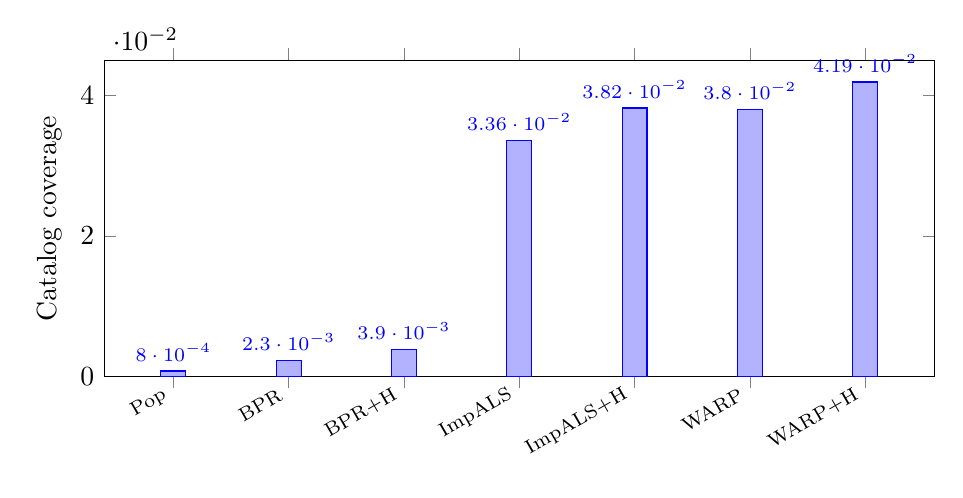
\begin{tikzpicture}
    \begin{axis}[
      ybar,
      bar width=9pt,
      ymin=0,
      ymax=0.045,
      ylabel={Catalog coverage},
      symbolic x coords={Pop,BPR,BPR+H,ImpALS,ImpALS+H,WARP,WARP+H},
      xtick=data,
      x tick label style={rotate=30,anchor=east,font=\scriptsize},
      width=\columnwidth,
      height=5.6cm,
      nodes near coords,
      every node near coord/.append style={font=\scriptsize},
    ]
    \addplot coordinates {
      (Pop,0.0008)
      (BPR,0.0023)
      (BPR+H,0.0039)
      (ImpALS,0.0336)
      (ImpALS+H,0.0382)
      (WARP,0.0380)
      (WARP+H,0.0419)
    };
    \end{axis}
  \end{tikzpicture}
  \caption{Catalog-coverage comparison for the main ranking models and their hybrid variants.}
  \label{fig:coveragebars}
\end{figure}

\subsection{Cold-start and subgroup behavior}
The cold-vs.-warm comparison in Table~\ref{tab:coldwarm} shows that subgroup behavior is not uniform across models. The popularity baseline and plain BPR remain clearly worse for cold users than for warm users. By contrast, the hybrid reranker helps BPR substantially on the cold-user slice, while Implicit ALS and WARP already perform strongly enough that the hybrid layer mainly changes the balance between subgroup strength and overall breadth rather than simply improving every metric at once.

\begin{table}[t]
  \caption{Cold-user vs.\ warm-user NDCG@10. Positive gap means warm users outperform cold users; negative gap means the cold-user slice scored higher in this benchmark sample.}
  \label{tab:coldwarm}
  \centering
  \footnotesize
  \setlength{\tabcolsep}{5pt}
  \resizebox{\columnwidth}{!}{%
  \begin{tabular}{@{}lrrr@{}}
    \toprule
    Model & Cold NDCG@10 $\uparrow$ & Warm NDCG@10 $\uparrow$ & Gap \\
    \midrule
    Popularity baseline & 0.0013 & 0.0061 & 0.0048 \\
    BPR (custom PyTorch) & 0.0011 & 0.0063 & 0.0052 \\
    BPR + content hybrid & 0.0083 & 0.0063 & -0.0020 \\
    Implicit ALS & \textbf{0.1282} & 0.0677 & -0.0605 \\
    Implicit ALS + content hybrid & 0.1129 & 0.0683 & -0.0447 \\
    WARP (custom PyTorch) & 0.1038 & 0.0445 & -0.0593 \\
    WARP + content hybrid & 0.1138 & 0.0480 & -0.0658 \\
    \bottomrule
  \end{tabular}
  }
\end{table}

\subsection{Hybrid reranking effects}
The hybrid wrapper is most useful when read as a controlled comparison against the same base candidate pool. Table~\ref{tab:hybriddelta} shows that every hybrid variant improves coverage, but the accuracy trade-off depends on the base recommender. In this table, positive deltas mean the hybrid layer improved the metric relative to the base recommender, while negative deltas mean the hybrid layer reduced that metric. BPR and WARP benefit on both NDCG and cold-user NDCG, while Implicit ALS gives up a small amount of NDCG in exchange for a broader recommendation footprint. Figure~\ref{fig:ndcgbars} makes the main ranking-quality differences visually clearer than the raw table alone.

\begin{table}[t]
  \caption{Hybrid-vs.-base deltas. The hybrid wrapper broadens coverage across all reported base recommenders, but the effect on NDCG depends on the underlying collaborative model.}
  \label{tab:hybriddelta}
  \centering
  \footnotesize
  \setlength{\tabcolsep}{4pt}
  \resizebox{\columnwidth}{!}{%
  \begin{tabular}{@{}lrrrrr@{}}
    \toprule
    Base model & Base NDCG & Hybrid NDCG & $\Delta$NDCG & $\Delta$Coverage & $\Delta$Cold NDCG \\
    \midrule
    BPR (custom PyTorch) & 0.0079 & 0.0090 & +0.0011 & +0.0016 & +0.0072 \\
    BPR (\texttt{implicit}) & 0.0021 & 0.0028 & +0.0007 & +0.0012 & +0.0005 \\
    Implicit ALS & 0.0674 & 0.0635 & -0.0039 & +0.0047 & -0.0153 \\
    WARP (custom PyTorch) & 0.0478 & 0.0500 & +0.0021 & +0.0039 & +0.0100 \\
    \bottomrule
  \end{tabular}
  }
\end{table}

\begin{figure}[t]
  \centering
  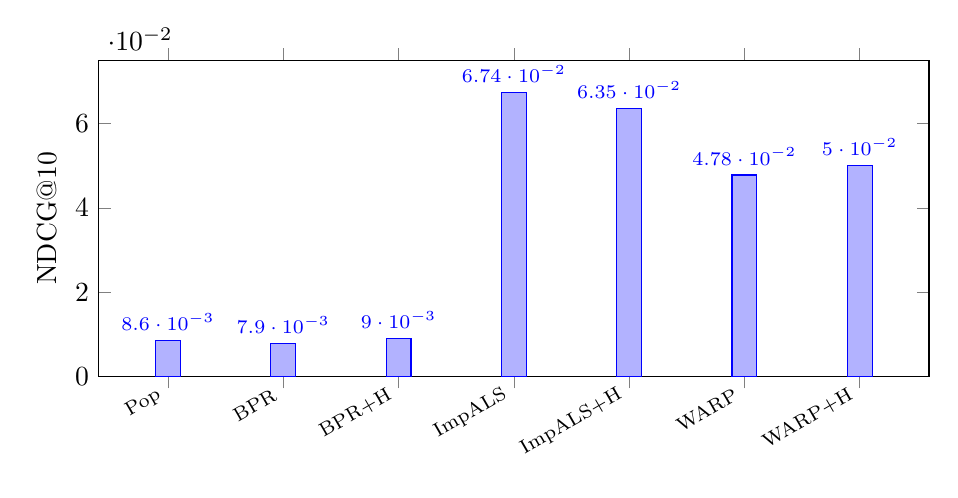
\begin{tikzpicture}
    \begin{axis}[
      ybar,
      bar width=9pt,
      ymin=0,
      ymax=0.075,
      ylabel={NDCG@10},
      symbolic x coords={Pop,BPR,BPR+H,ImpALS,ImpALS+H,WARP,WARP+H},
      xtick=data,
      x tick label style={rotate=30,anchor=east,font=\scriptsize},
      width=\columnwidth,
      height=5.6cm,
      nodes near coords,
      every node near coord/.append style={font=\scriptsize},
    ]
    \addplot coordinates {
      (Pop,0.0086)
      (BPR,0.0079)
      (BPR+H,0.0090)
      (ImpALS,0.0674)
      (ImpALS+H,0.0635)
      (WARP,0.0478)
      (WARP+H,0.0500)
    };
    \end{axis}
  \end{tikzpicture}
  \caption{NDCG@10 comparison for the main ranking models and their hybrid variants.}
  \label{fig:ndcgbars}
\end{figure}

\subsection{Discussion}
\textbf{Rating vs.\ ranking mismatch.} MF achieves the best RMSE/MAE among reported rating predictors, yet Top-$N$ quality is dominated by models trained with ranking-aware losses (Table~\ref{tab:rank}), consistent with prior work on evaluation alignment~\cite{cremonesi2010}. \textbf{Strongest overall ranker.} Implicit ALS remains the best pure collaborative model on NDCG@10, Precision@10, and Recall@10, which is also visible in Figure~\ref{fig:ndcgbars}. \textbf{Breadth vs.\ sharpness.} Table~\ref{tab:beyond} shows that stronger recommenders are not only more accurate; they also cover much more of the catalog than the popularity baseline. WARP plus the hybrid layer reaches the highest coverage, while BPR produces the highest novelty. \textbf{Cold-start behavior.} Table~\ref{tab:coldwarm} shows that the content hybrid is especially helpful for the weaker BPR family, where cold-user NDCG rises sharply. For Implicit ALS, however, the hybrid wrapper trades a small amount of ranking quality for wider catalog coverage. \textbf{Refactor value:} the main contribution of the upgraded system is not replacing every baseline, but making the relationship among scoring, recommendation, explanation, and analysis explicit enough to support new project questions safely.

\subsection{Extension-layer observations}
The refactored project now supports analyses that were not available in the original baseline. First, each recommendation can be accompanied by structured support signals and a weakening condition, which makes the ranking output easier to inspect and present. Second, fairness and cold-start summaries reveal whether performance concentrates on heavy users or degrades for sparse-user slices. Third, beyond-accuracy metrics expose whether a model is broad, repetitive, or overly popularity-driven. Finally, the optional content-aware hybrid reranker creates a concrete path for comparing collaborative-only and collaborative-plus-content behavior without retraining the core recommenders. Table~\ref{tab:hybriddelta} makes this trade-off explicit: every hybrid variant broadens coverage, but only some models gain both accuracy and cold-user quality at the same time.

\subsection{Qualitative explanation example}
The explainability layer is easiest to understand through a concrete recommendation. For one user in the demo, the system recommends a cutting-die accessory because the user previously interacted with several paper-craft and die-cutting products. The explanation module then surfaces (i) supporting history items from the same craft-tool cluster, (ii) similar supporting catalog items, (iii) a support confidence score summarizing how strongly those signals align with the recommendation, and (iv) a weakening condition stating that if the strongest support items were removed, the recommendation would likely fall below the displayed Top-$10$. This example illustrates the intended role of the extension: it does not retrain the base recommender, but it turns an otherwise opaque ranked item into a recommendation that can be inspected and discussed.

\subsection{Limitations and threats to validity}
Several limitations should be kept in mind when interpreting these results. First, the experiments are based on a single Amazon 5-core domain, so the observed trade-offs may not transfer directly to other categories with different interaction patterns. Second, all evaluation is offline; gains in NDCG, coverage, or cold-start behavior do not guarantee the same gains in real user satisfaction. Third, the explanation layer is post-hoc and approximate, so its weakening conditions should be read as practical diagnostics rather than causal proof. Fourth, the TF--IDF hybrid reranker is intentionally lightweight and may miss deeper semantic relationships that stronger text encoders could capture. Finally, the cold-start findings depend on the chosen activity thresholds and sampled evaluation slices, so they should be interpreted as benchmark summaries rather than universal statements about all sparse users.

\FloatBarrier

\section{Demo System}
We provide a Streamlit application (\texttt{streamlit run app/demo.py}) that exposes the pipeline in a presentation-friendly order instead of hiding everything behind a single recommendation list.

\paragraph{Primary recommendations and explanations.}
The demo first shows the user's profile and past activity, then the ranked candidate list, then the final Top-$N$ recommendations. Each displayed item can include product metadata, support confidence, supporting history items, similar support items, and a weakening statement that indicates what evidence removal would likely reduce its rank. These explanations are post-hoc and do not alter the base model's score.

\paragraph{Optional reranking layers.}
The interface supports two optional post-processing views. The first is a score-adjustment reranking toggle, which adjusts the base score using support confidence and a popularity penalty before resorting the same candidate pool. The second is a content-aware hybrid wrapper that reorders the collaborative candidate pool using TF--IDF review-profile similarity. Both layers remain optional and do not replace the baseline collaborative models.

\paragraph{Fairness audit.}
A dedicated section summarizes activity-bucket disparity, cold-user vs.\ warm-user NDCG, and a compact bucket table. This is an audit layer~\cite{li2021userfairness,burke2017multisided}, not a fairness-constrained learner.

\paragraph{Coverage and diversity snapshot.}
The demo also surfaces catalog coverage, diversity, novelty, and popularity-concentration style indicators so that users can see not only whether a model is accurate, but also whether it is narrow or repetitive.

\section{Reproducibility and Engineering}
Experiments are driven by \texttt{configs/default.yaml} and \texttt{configs/small.yaml}. Running \texttt{python main.py --config configs/default.yaml} executes preprocessing (if needed), training, evaluation, and writes JSON summaries under \texttt{experiments/}. The codebase also supports saving model artifacts for later evaluation-only runs. Preprocessing writes \texttt{verified} and \texttt{style} into train/test JSON when the raw record contains them. Unit tests now cover metrics, splitting behavior, recommendation-stage behavior, fairness summaries, counterfactual formatting, causal toggles, explanation evaluation, hybrid reranking, and cold-start summaries.

\section{Future Work and Feasible Extensions}
\label{sec:future}
The items below are scoped so a small team could implement them on this codebase without replacing the entire stack; they extend what we already ship rather than reproducing full systems from Section~2.1.

\begin{itemize}
  \item \textbf{Faster repeated reporting.} Cache hybrid-evaluation artifacts and extension-layer summaries so that repeated report-generation runs do not need to recompute every expensive recommendation pass.
  \item \textbf{Metadata-aware hybrid models.} Extend the content branch beyond TF--IDF review text to use product metadata such as brand, category, or ``also viewed'' relations when available.
  \item \textbf{Fairness-aware reranking.} Go beyond auditing by introducing a mild inference-time fairness re-ranker or sample-weighted training objective and comparing the resulting subgroup trade-offs~\cite{li2021userfairness}.
  \item \textbf{Improved natural-language explanations.} Turn the current structured support signals into more readable template-based text, while still keeping the explanation tied to concrete support evidence rather than a free-form language model.
  \item \textbf{Experimental sequential/transformer branch.} Implement a clearly isolated future-only experimental module inspired by sequential recommenders or PETER-style explainable transformers, without affecting the default baseline pipeline.
  \item \textbf{Persistence and demo latency.} Persist text-profile artifacts and optional embedding caches so the demo starts faster and can be shown reliably during presentations.
\end{itemize}

\section{Conclusion}
We implemented a recommender project pipeline on an Amazon 5-core domain with the required preprocessing, rating prediction metrics, Top-10 ranking metrics, and an interactive demo. Empirically, \textbf{matrix factorization} is strongest on RMSE/MAE, while \textbf{implicit ALS} and \textbf{custom WARP} deliver the best documented Top-10 NDCG, illustrating the importance of matching training objectives to evaluation tasks~\cite{cremonesi2010,hu2008collaborative}. The main upgrade is architectural: the project now cleanly separates rating prediction, ranking, recommendation extraction, explanation, and post-hoc analysis, making it safer to extend and easier to report. On top of the preserved baselines, we now support structured counterfactual explanations, score-adjusted reranking, fairness and beyond-accuracy auditing, cold-start benchmarking, and an optional content-aware hybrid branch. These additions make the system substantially more transparent without discarding the original working models.

\section*{Acknowledgments}
Course staff and open-source maintainers of PyTorch, SciPy, scikit-learn, and \texttt{implicit}.

\begin{thebibliography}{99}

\bibitem{amazon5core}
J.~Ni, J.~Li, and J.~McAuley.
\newblock Amazon Review Data (2018).
\newblock \url{https://nijianmo.github.io/amazon/index.html}.

\bibitem{cremonesi2010}
P.~Cremonesi, Y.~Koren, and R.~Turrin.
\newblock Performance of recommender algorithms on top-$N$ recommendation tasks.
\newblock In \emph{Proceedings of the Fourth ACM Conference on Recommender Systems (RecSys)}, 2010.

\bibitem{herlocker2004evaluating}
J.~L. Herlocker, J.~A. Konstan, L.~G. Terveen, and J.~T. Riedl.
\newblock Evaluating collaborative filtering recommender systems.
\newblock \emph{ACM Transactions on Information Systems (TOIS)} 22(1), 5--53, 2004.

\bibitem{hu2008collaborative}
Y.~Hu, Y.~Koren, and C.~Volinsky.
\newblock Collaborative filtering for implicit feedback datasets.
\newblock In \emph{Proceedings of the 8th IEEE International Conference on Data Mining (ICDM)}, 263--272, 2008.

\bibitem{rendle2009bpr}
S.~Rendle, C.~Freudenthaler, Z.~Gantner, and L.~Schmidt-Thieme.
\newblock {BPR}: Bayesian personalized ranking from implicit feedback.
\newblock In \emph{Proceedings of the 25th Conference on Uncertainty in Artificial Intelligence (UAI)}, 452--461, 2009.

\bibitem{koren2009matrix}
Y.~Koren, R.~Bell, and C.~Volinsky.
\newblock Matrix factorization techniques for recommender systems.
\newblock \emph{Computer} 42(8), 30--37, 2009.

\bibitem{weston2011wsabie}
J.~Weston, S.~Bengio, and N.~Usunier.
\newblock {WSABIE}: Scaling up to large vocabulary image annotation.
\newblock In \emph{Proceedings of the Twenty-Second International Joint Conference on Artificial Intelligence (IJCAI)}, 2764--2770, 2011.

\bibitem{he2017neural}
X.~He, L.~Liao, H.~Zhang, L.~Nie, X.~Hu, and T.-S. Chua.
\newblock Neural collaborative filtering.
\newblock In \emph{Proceedings of the 26th International Conference on World Wide Web (WWW)}, 173--182, 2017.

\bibitem{mcauley2013hidden}
J.~McAuley and J.~Leskovec.
\newblock Hidden factors and hidden topics: understanding rating dimensions with review text.
\newblock In \emph{Proceedings of the 7th ACM Conference on Recommender Systems (RecSys)}, 165--172, 2013.

\bibitem{reimers2019sentence}
N.~Reimers and I.~Gurevych.
\newblock Sentence-{BERT}: Sentence embeddings using {Siamese} {BERT}-networks.
\newblock In \emph{Proceedings of the 2019 Conference on Empirical Methods in Natural Language Processing (EMNLP)}, 3982--3992, 2019.

\bibitem{zhang2020explainable}
Y.~Zhang and X.~Chen.
\newblock Explainable recommendation: A survey and new perspectives.
\newblock \emph{ACM Computing Surveys (CSUR)} 52(1), Article~5, 1--38, 2020.

\bibitem{burke2017multisided}
R.~Burke.
\newblock Multisided fairness for recommendation.
\newblock \emph{arXiv preprint arXiv:1707.00093}, 2017.

\bibitem{zhang2017heterogeneous}
Y.~Zhang, Q.~Ai, X.~Chen, and W.~B. Croft.
\newblock Joint representation learning for top-$N$ recommendation with heterogeneous information sources.
\newblock In \emph{Proceedings of the 26th ACM International Conference on Information and Knowledge Management (CIKM)}, 1449--1458, 2017.
\newblock \url{https://doi.org/10.1145/3132847.3132892}

\bibitem{zhang2018conversational}
Y.~Zhang, X.~Chen, Q.~Ai, L.~Yang, and W.~B. Croft.
\newblock Towards conversational search and recommendation: System ask, user respond.
\newblock In \emph{Proceedings of the 27th ACM International Conference on Information and Knowledge Management (CIKM)}, 177--186, 2018.
\newblock \url{https://doi.org/10.1145/3269206.3271776}

\bibitem{geng2022p5}
S.~Geng, Z.~Fu, J.~Tan, Y.~Ge, G.~de Melo, and Y.~Zhang.
\newblock Recommendation as language processing (RLP): A unified pretrain, personalized prompt and predict paradigm (P5).
\newblock \emph{arXiv preprint arXiv:2203.13366}, 2022.

\bibitem{chen2020neuralreasoning}
X.~Chen, H.~Xu, Y.~Zhang, J.~Tang, Y.~Cao, Z.~Qin, and H.~Zha.
\newblock Neural collaborative reasoning.
\newblock In \emph{Proceedings of the European Conference on Machine Learning and Principles and Practice of Knowledge Discovery in Databases (ECML PKDD)}, 2020.
\newblock \url{https://arxiv.org/abs/2005.08129}

\bibitem{xu2021causal}
S.~Xu, Y.~Ge, Y.~Li, Z.~Fu, X.~Chen, and Y.~Zhang.
\newblock Causal collaborative filtering.
\newblock \emph{arXiv preprint arXiv:2102.01868}, 2021.

\bibitem{li2021userfairness}
Y.~Li, H.~Chen, Z.~Fu, Y.~Ge, and Y.~Zhang.
\newblock User-oriented fairness in recommendation.
\newblock \emph{arXiv preprint arXiv:2104.10671}, 2021.

\bibitem{li2021pextransformer}
L.~Li, Y.~Zhang, and L.~Chen.
\newblock Personalized transformer for explainable recommendation.
\newblock In \emph{Proceedings of the 59th Annual Meeting of the Association for Computational Linguistics (ACL)}, 4947--4960, 2021.
\newblock \url{https://aclanthology.org/2021.acl-long.383/}

\bibitem{tan2021counterfactual}
J.~Tan, S.~Xu, Y.~Ge, Y.~Li, X.~Chen, and Y.~Zhang.
\newblock Counterfactual explainable recommendation.
\newblock In \emph{Proceedings of the 30th ACM International Conference on Information and Knowledge Management (CIKM)}, 3124--3133, 2021.
\newblock \url{https://arxiv.org/abs/2108.10539}

\end{thebibliography}

\end{document}
